\documentclass{article}

\usepackage{graphicx}
\usepackage{tikz}
\usepackage{tikzsymbols}
\usetikzlibrary{calc,patterns,shapes.geometric}
\pagestyle{empty}
\usepackage[margin=0pt]{geometry}
\geometry{papersize={14in,12in}}

\def\centerarc[#1](#2)(#3:#4:#5){\draw[#1] ($(#2)+({#5*cos(#3)},{#5*sin(#3)})$) arc (#3:#4:#5);}

\begin{document}
	\begin{figure}
		\centering
		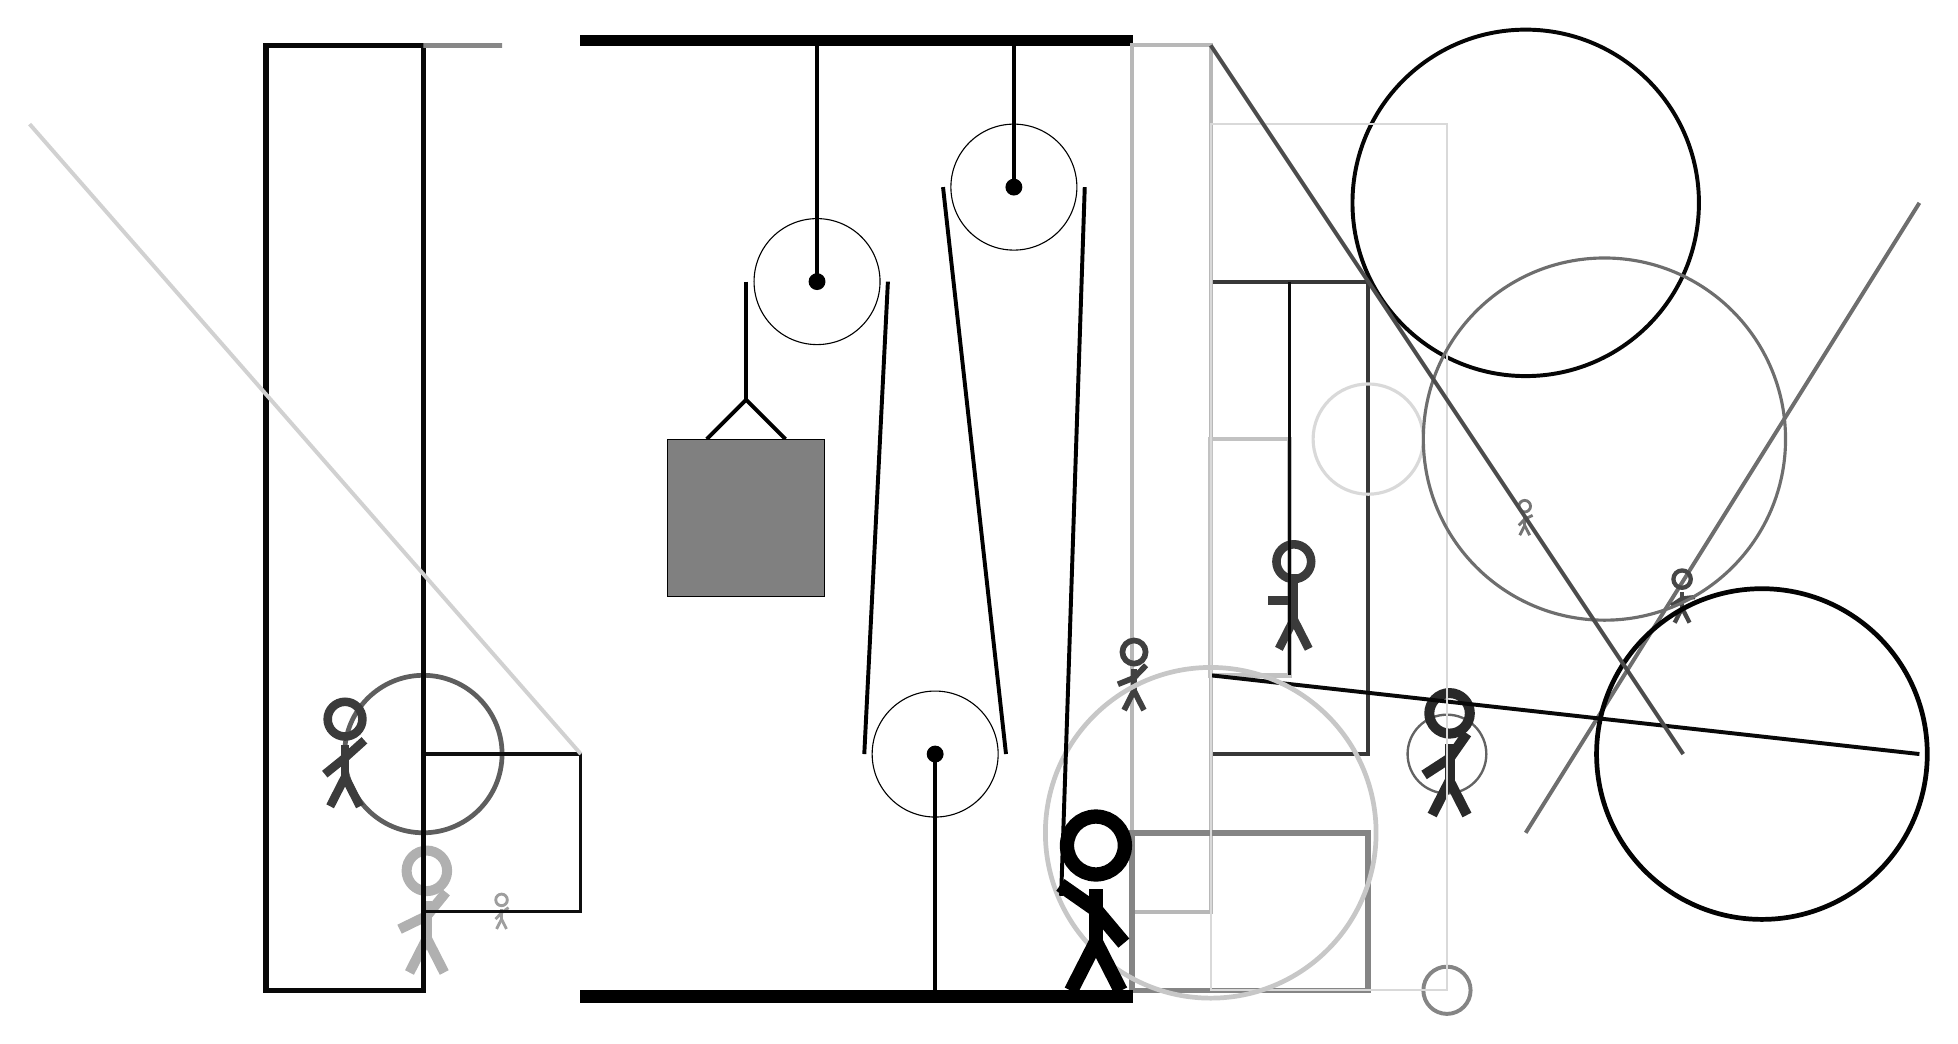
\begin{tikzpicture}
			%%%%% START %%%%%
			
			\draw[fill=black] (-2, 9) rectangle (5, 9.125);
			
			\draw (1, 6) circle (0.8);
			\draw[fill=black] (1, 6) circle (0.1);
			\draw[line width=0.5mm]  (1, 9) -- (1, 6);
			
			\draw[fill=white](2.5, 0) circle (0.8);
			\draw[fill=black] (2.5, 0) circle (0.1);
			\draw[line width=0.5mm]  (2.5, -3) -- (2.5, 0);
			
			\draw[fill=white](3.5, 7.2) circle (0.8);
			\draw[fill=black] (3.5, 7.2) circle (0.1);
			\draw[line width=0.5mm] (3.5, 9) -- (3.5, 7.2);
			
			\draw[line width=0.5mm] (-0.4, 4.0) -- (0.1, 4.5) -- (0.6, 4.0);
			\draw[fill=black!50] (-0.9, 4.0) rectangle (1.1, 2.0);
			
			\draw[line width=0.5mm, color=black!57](10, -1) -- (15, 7);
			
			\draw[line width=0.4mm, color=black!18] (5, 1) rectangle (5, 6);
			\draw[line width=0.5mm, color=black!78] (6, 0) rectangle (8, 6);
			\node[line width=0.4mm, color=black!38] at (-3, -2) {\Strichmaxerl[2][47][36]};
			\draw [line width=0.5mm, color=black!48](9, -3) circle (0.3);
			
			\draw [line width=0.6mm, color=black!63](-4, 0) circle (1.0);
			\node[line width=0.5mm, color=black!77] at (-5, 0) {\Strichmaxerl[6][39][42]};
			\draw[line width=0.5mm, color=black!28] (5, 9) rectangle (6, -2);
			\draw [line width=0.3mm, color=black!61](9, 0) circle (0.5);
			
			\node[line width=0.7mm, color=black!54] at (10, 3) {\Strichmaxerl[2][47][25]};
			\node[line width=0.2mm, color=black!31] at (-4, -2) {\Strichmaxerl[7][26][51]};
			\node[line width=0.7mm, color=black!72] at (12, 2) {\Strichmaxerl[3][34][6]};
			\node[line width=0.7mm, color=black!84] at (9, 0) {\Strichmaxerl[7][33][55]};
			\draw [line width=0.4mm, color=black!15](8, 4) circle (0.7);
			\draw[line width=0.4mm, color=black!94] (-4, 0) rectangle (-2, -2);
			\draw[line width=0.7mm, color=black!48] (5, -1) rectangle (8, -3);
			
			\draw[line width=0.2mm, color=black!47] (-4, 0) rectangle (-4, -3);
			\draw [line width=0.5mm, color=black!98](10, 7) circle (2.2);
			\draw [line width=0.6mm, color=black!99](13, 0) circle (2.1);
			\draw[line width=0.6mm, color=black!24] (6, 4) rectangle (7, 1);
			\draw[line width=0.7mm, color=black!97] (-4, -3) rectangle (-6, 9);
			
			\draw[line width=0.5mm, color=black!97](6, 1) -- (15, 0);
			
			\draw[line width=0.2mm, color=black!15] (6, -3) rectangle (9, 8);
			\node[line width=0.7mm, color=black!77] at (7, 2) {\Strichmaxerl[6][0][90]};
			\draw[line width=0.5mm, color=black!18](-2, 0) -- (-9, 8);
			\node[line width=0.4mm, color=black!75] at (5, 1) {\Strichmaxerl[4][22][46]};
			\draw [line width=0.4mm, color=black!57](11, 4) circle (2.3);
			\draw[line width=0.5mm, color=black!96](7, 6) -- (7, 1);
			
			\draw [line width=0.6mm, color=black!22](6, -1) circle (2.1);
			\draw[line width=0.6mm, color=black!47] (-3, 9) rectangle (-4, 9);
			\draw[line width=0.5mm, color=black!70](6, 9) -- (12, 0);
			
			\draw[line width=0.5mm] (0.1, 6) -- (0.1, 4.5);
			\centerarc[line width=0.5mm](1, 6)(0:180:0.9);
			\draw[line width=0.5mm](1.9, 6) -- (1.6, 0);
			\centerarc[line width=0.5mm](2.5, 0)(180:360:0.9);
			\draw[line width=0.5mm](3.4, 0) -- (2.6, 7.2);
			\centerarc[line width=0.5mm](3.5, 7.2)(0:180:0.9);
			\draw[line width=0.5mm](4.4, 7.2) -- (4.1, -1.8);
			
			\node at (4.5, -1.9) {\Strichmaxerl[10][-35][-50]};
			
			\draw[fill=black] (-2, -3) rectangle (5, -3.15);
			
			%%%%% END %%%%%
		\end{tikzpicture}
	\end{figure}	
\end{document}